\begin{blocksection}
Synchronous Digital Systems (SDSs) are systems designed to process input as it comes in and output it as quickly as it comes in.  The input is always a series of pins with either high or low voltage, and the output is another series of pins, each with either high or low voltage.  A clock is used to tell the input and output when to switch to the next value; the switch always occurs on the rising edge (low to high voltage) of the clock.  This is so that the output is always consistent, otherwise halfway through the switch of the input, the output might be based on the old input or the new, depending on the quality of the circuit and also some random chance based on electron movement.  Note: the output always takes a small amount of time to stabilize after the rising edge.

When slowed down, clock cycles will look something like below.  This is three clock cycles in a row, and here is the rising edge:

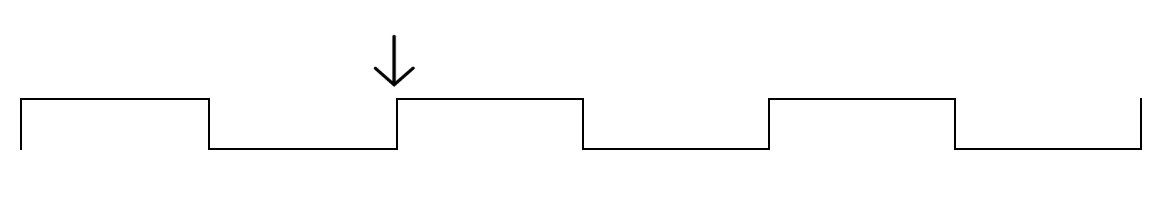
\includegraphics[width=\textwidth]{sds/explanation}

\end{blocksection}